%--------------------------------------------------------------------------------------------
% MPAS-A Overview
%--------------------------------------------------------------------------------------------

\chapter{MPAS-A Overview}
\label{chap:atmosphere_overview}

The Model for Prediction Across Scales -- Atmosphere (MPAS-A) is a
non-hydrostatic atmosphere model that is part of a family of
Earth-system component models, collectively known as MPAS.  All MPAS
models have in common their use of centoidal Voronoi tessellations for
their horizontal meshes, which has motivated the development of a common
software framework that provides a high-level driver program and
infrastructure for providing parallel execution, input and output, and
other software infrastructure.

\section{Features}

Key features of MPAS-A include:

\begin{itemize}
\item Fully-compressible, non-hydrostatic dynamics
\item Split-explicit Runge-Kutta time integration
\item something,
\item something,
\item something.
\end{itemize}

At present, MPAS-A includes parameterizations of physical processes
taken from the Weather Research and Forecasting (WRF) Model
\footnote{\url{http://www.wrf-model.org/}.}. Specifically, MPAS-A has
support for:

\begin{itemize}
\item Radiation: CAM and RRTMG long-wave and short-wave radiation schemes
\item Land-surface: NOAH land-surface model
\item Surface-layer: Monin-Obukhov
\item Boundary-layer: YSU PBL scheme
\item Convection: Kain-Fritsch and Tiedtke convection parameterizations
\item Cloud microphysics: WSM6 and Kessler schemes
\end{itemize}

\section{Model components}

MPAS-A employs two main components: the model itself, which includes
atmospheric dynamics and physics; and an initialization component for
generating initial conditions and update files for sea-surface
temperature and sea ice. Both of these components are built as ``cores''
within the MPAS software framework and make use of the same driver
program and software infrastructure, but are compiled separately as
distinct executables. 

\begin{figure}[htb]
\begin{center}
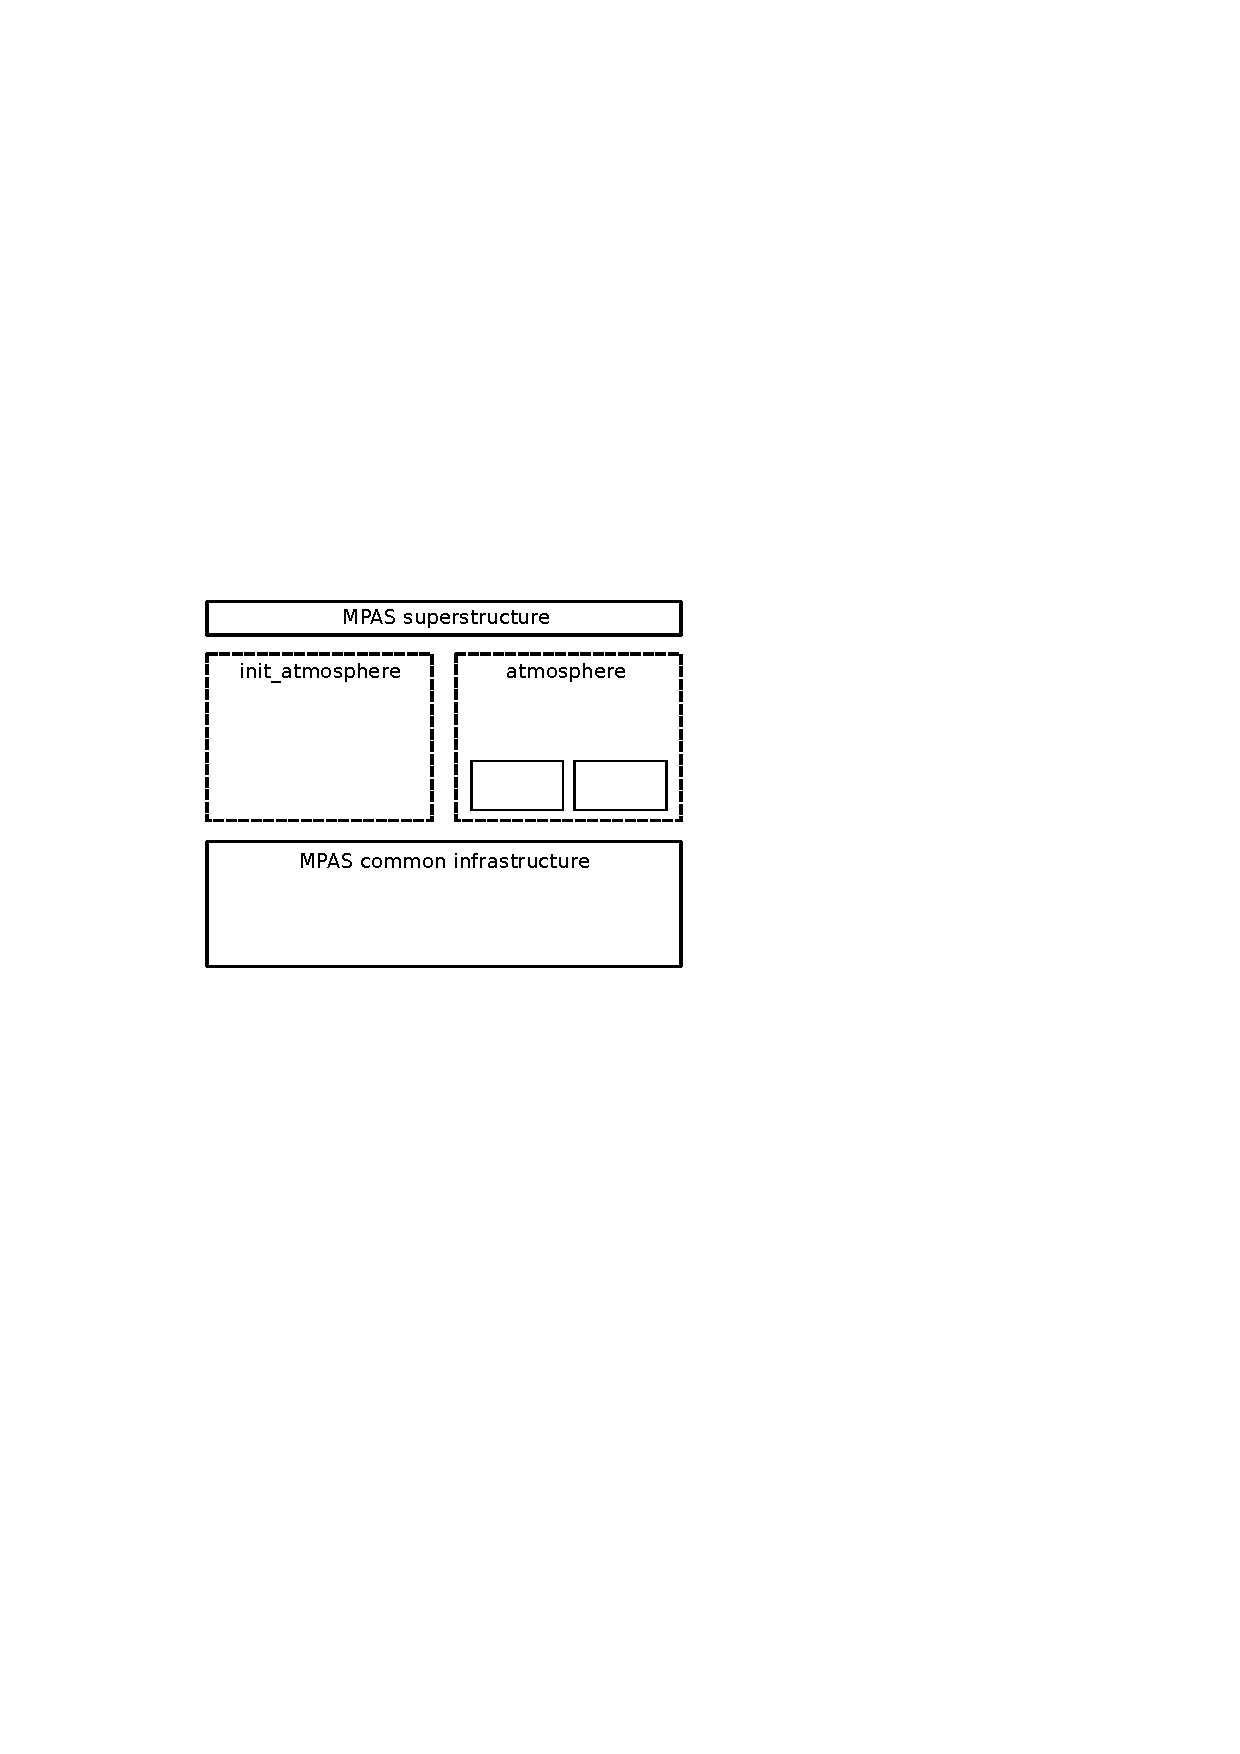
\includegraphics[width=3.5in]{atmosphere/figures/mpas-a_components.pdf}
\caption{Blah.}
\label{fig:atm_components}
\end{center}
\end{figure}

The details of compiling these components are given in Chapter
\ref{chap:mpas_build_instructions}, and the basic steps to create initial
conditions and run the MPAS-A model are outlined in Chapter
\ref{chap:running_mpas_a}.
